% =============================================================================
% Section 2 — Kinetic Proofreading
% =============================================================================
\section{Kinetic Proofreading: How a Cell Buys Accuracy}\label{sec:proofreading}

\begin{objectives}
\begin{itemize}[leftmargin=*,itemsep=1pt,topsep=1pt]
  \item Derive the equilibrium discrimination limit from a free-energy difference.
  \item Show why that limit is catastrophic at genome scale, and how irreversible delay stages beat it.
  \item Prove that adding stages never raises the error rate, and that $k$ extra stages buy exactly $\gamma^k$.
  \item Reproduce the error cascade numerically and read it off a 3D surface.
\end{itemize}
\end{objectives}

\subsection{Biological setting}

DNA polymerase~$\varepsilon$ replicates the leading strand of the human nuclear
genome. Its catalytic subunit is \texttt{POLE}: UniProt \texttt{Q07864},
$2286$~residues, encoded at Ensembl \texttt{ENSG00000177084} on chromosome~12 in
GRCh38. At every position it must choose between the correct incoming nucleotide
and three incorrect ones.

The thermodynamic discrimination available is small. The free-energy difference
between a correct Watson--Crick pair and a mismatch is
$\Delta\Delta G \approx 4.6\,k_BT$, giving an equilibrium error ratio
\begin{equation}\label{eq:gamma0}
  \gamma_0 \;=\; e^{-\Delta\Delta G/k_BT} \;\approx\; 10^{-2}.
\end{equation}
One error per hundred bases. A human genome is $3.1\times10^9$ bases; at that
rate replication would introduce some $3\times10^7$ errors per round, which no
organism survives. Yet the measured rate is near $10^{-10}$ per base per
division. Eight orders of magnitude are unaccounted for.

Hopfield (1974) and Ninio (1975) supplied the missing idea: the cell does not
play the equilibrium game. It spends energy to run the discrimination step more
than once.

\subsection{Mathematical development}

\begin{model}[Multiplicative stages]\label{model:stages}
The enzyme applies $m$ discrimination stages in series. Each stage is driven
irreversibly (by NTP hydrolysis), resets the comparison, and lets a wrong
substrate through with probability $\gamma \in (0,1)$, independently of the others.
\end{model}

Independence is the substantive assumption, and we will return to it: it is the
hypothesis that Section~3's no-go theorem turns against the model.

Under Assumption~\ref{model:stages} the probability that a wrong substrate
survives all $m$ stages is a product of $m$ independent events:
\begin{equation}\label{eq:cascade}
  \mathcal{E}_m(\gamma) \;=\; \underbrace{\gamma \cdot \gamma \cdots \gamma}_{m} \;=\; \gamma^m .
\end{equation}

Two consequences follow immediately, and both are formalised below.

\begin{proposition}[Monotonicity]\label{prop:antitone}
For $\gamma \in [0,1]$ and $n \le m$, $\;\gamma^m \le \gamma^n$. Adding stages
never raises the error rate.
\end{proposition}

\begin{proof}
Write $\gamma^m = \gamma^n \cdot \gamma^{m-n}$. Since $0 \le \gamma \le 1$ we have
$0 \le \gamma^{m-n} \le 1$, and multiplying the non-negative quantity $\gamma^n$
by a factor in $[0,1]$ cannot increase it.
\end{proof}

\begin{proposition}[Discrimination gain]\label{prop:gain}
For $\gamma \ne 0$ and any $n, k$, $\;\gamma^{n+k}/\gamma^{n} = \gamma^{k}$: each
additional stage multiplies the discrimination by $\gamma$, regardless of how
many stages precede it.
\end{proposition}

\begin{proof}
$\gamma^{n+k} = \gamma^{n}\gamma^{k}$ by the law of exponents, and dividing by
$\gamma^{n} \ne 0$ leaves $\gamma^{k}$.
\end{proof}

Proposition~\ref{prop:gain} is what makes the scheme powerful: the returns are
geometric, not diminishing. Three stages at $\gamma = 10^{-2}$ give
$\mathcal{E}_3 = 10^{-6}$, and the remaining gap to the observed $10^{-10}$ is
closed downstream by mismatch repair --- the subject of Section~5, and, as it
turns out, the place where the mechanism of Section~4 actually lives.

\subsection{Formalisation}

The two propositions are checked in \file{formal/ANSE/GeneticsTextbook.lean}.

\begin{lstlisting}
theorem error_antitone (γ : ℝ) (h0 : 0 ≤ γ) (h1 : γ ≤ 1) {m n : ℕ} (hnm : n ≤ m) :
    γ ^ m ≤ γ ^ n :=
  pow_le_pow_of_le_one h0 h1 hnm

theorem discrimination_gain (γ : ℝ) (hγ : γ ≠ 0) (n k : ℕ) :
    γ ^ (n + k) / γ ^ n = γ ^ k := by
  rw [pow_add, mul_comm, mul_div_assoc, div_self (pow_ne_zero n hγ), mul_one]
\end{lstlisting}

\noindent
Note what the hypotheses are doing. \lean{error_antitone} needs
$0 \le \gamma \le 1$: a ``stage'' that let wrong substrates through \emph{more}
often than it rejected them would make the product grow. \lean{discrimination_gain}
needs only $\gamma \ne 0$, because it is a statement about exponents and not
about probabilities at all. Hypotheses that are not needed are not assumed; this
is a habit worth acquiring, because an unnecessary hypothesis hides which
assumption your conclusion really rests on.

\begin{numerics}[2.1]
\file{scripts/textbook/make_figures.py}, section~2. With $\gamma = 10^{-2}$ and
$m = 3$, evaluating \eqref{eq:cascade} in exact rational arithmetic gives
$\mathcal{E}_3 = 1/1\,000\,000$ exactly, matching the Lean constant evaluation
\lean{three_stage_error_control}. Figure~\ref{fig:cascade} plots
$\log_{10}\mathcal{E}_m(\gamma)$ over $\gamma \in [0.005, 0.6]$, $m \in \{1,\dots,6\}$.
\end{numerics}

\begin{figure}[htbp]
  \centering
  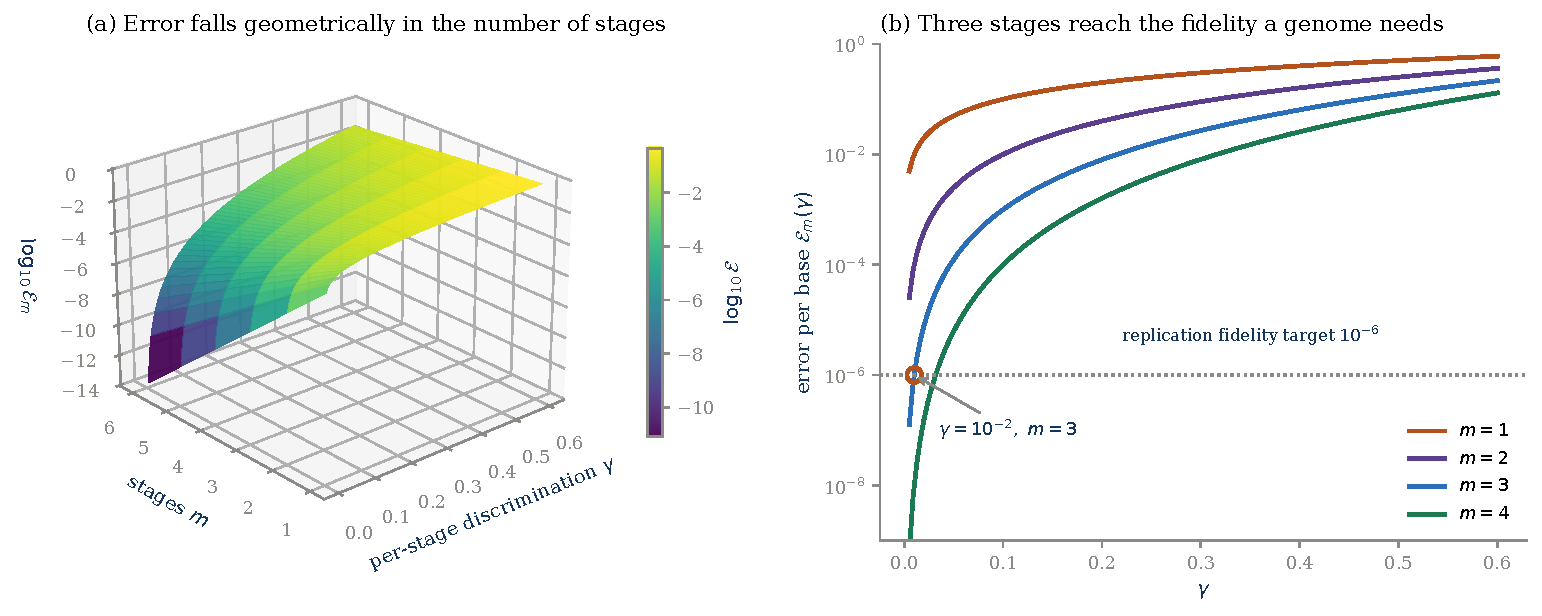
\includegraphics[width=\textwidth]{fig02_proofreading_cascade.pdf}
  \caption{(a) The error surface $\log_{10}\mathcal{E}_m(\gamma) = m\log_{10}\gamma$.
  Because the dependence on $m$ is linear in the logarithm, the surface is a
  family of straight lines --- which is the geometric return of
  Proposition~\ref{prop:gain} seen edge-on. (b) Sections at fixed $m$. The circled
  point is the biologically relevant corner: three stages at $\gamma = 10^{-2}$
  reach $10^{-6}$, within reach of the fidelity a genome needs once downstream
  repair is included.}
  \label{fig:cascade}
\end{figure}

\subsection{Where the model is vulnerable}

Assumption~\ref{model:stages} contains three separable claims, and it is worth
naming them now because Sections~3--5 attack them in turn:

\begin{enumerate}[leftmargin=*,itemsep=1pt]
  \item \emph{Multiplicativity} --- stages compose by multiplication.
  \item \emph{Range} --- each per-stage factor lies in $[0,1]$.
  \item \emph{Isolation} --- the error rate the cell experiences is the error rate
        the enzyme produces; nothing downstream intervenes.
\end{enumerate}

Claims (1) and (2) are mild and are what Section~3's no-go theorem assumes.
Claim (3) is strong, usually unstated, and false. Section~5 is about what happens
when you drop it.

\begin{worked}[2.2: how many stages does a genome need?]
\textbf{Problem.} Taking $\gamma = 10^{-2}$ and demanding a per-base error below
$10^{-9}$ from proofreading alone, how many stages are required? What does the
answer suggest about the biology?

\textbf{Solution.} We need $\gamma^m < 10^{-9}$, i.e.\ $10^{-2m} < 10^{-9}$, i.e.\
$2m > 9$, so $m \ge 5$.

Real replicative polymerases have one proofreading exonuclease, not five. The
model therefore cannot reach observed fidelity by stages alone, \emph{and it does
not claim to}: the shortfall is made up by mismatch repair acting after the
polymerase has moved on. The exercise is worth doing because it shows the gap is
structural --- any account of replication fidelity must include a downstream step,
which is precisely the term that Section~5 will show the data force upon us.
\end{worked}

\begin{exercise}
Using Proposition~\ref{prop:gain}, show that the discrimination gained by going
from $m$ to $m+1$ stages is independent of $m$. Why is this surprising when
compared with most engineering error-correction schemes, where returns diminish?
\end{exercise}

\begin{exercise}
Suppose stages are \emph{not} independent: passing stage~1 makes passing stage~2
more likely, so that $\mathcal{E}_2 = \gamma^2 + c$ for some $c > 0$. Show that
Proposition~\ref{prop:antitone} can fail. What does this tell you about the role
of the independence assumption?
\end{exercise}

\begin{exercise}
The equilibrium bound \eqref{eq:gamma0} assumes discrimination comes only from
$\Delta\Delta G$ at a single binding step. Compute the $\Delta\Delta G$ that would
be required to reach $\gamma = 10^{-6}$ in one step, in units of $k_BT$ and in
$\mathrm{kJ\,mol^{-1}}$ at $310$\,K. Comment on whether a hydrogen-bonded base pair
could plausibly supply it.
\end{exercise}

\begin{ledger}
\textbf{Measured:} $\Delta\Delta G \approx 4.6\,k_BT$ for Watson--Crick
discrimination (standard thermodynamic estimate); observed replication fidelity
$\sim10^{-10}$ per base per division. Gene and protein identifiers retrieved live
from Ensembl and UniProt (\file{textbook/data/genomic_records.json}). \\
\textbf{Assumed:} Assumption~\ref{model:stages} --- multiplicativity, per-stage
factors in $[0,1]$, and isolation from downstream repair. The third is false and
is dropped in Section~5. \\
\textbf{Proved:} Propositions~\ref{prop:antitone} and~\ref{prop:gain}
(\lean{error_antitone}, \lean{discrimination_gain}), and
$\left(10^{-2}\right)^3 = 10^{-6}$ (\lean{three_stage_error_control}). Gate:
clean, no \lean{sorryAx}. \\
\textbf{Open:} the per-stage factor $\gamma$ is treated as a single number for a
process that is in reality nucleotide- and context-dependent. No measurement in
this book constrains that variation.
\end{ledger}
